\section{Results}

The optimization problem was solved using \(N=200\) shooting intervals. IPOPT converged successfully after 357 iterations, requiring approximately \(8.0~\mathrm{s}\) of computation time. The solver returned the status \texttt{Solve\_Succeeded}. The optimal lap time obtained was

\begin{equation}
    T^*=61.665~\mathrm{s}.
\end{equation}

The main numerical results are summarized in Table~\ref{tab:optimization_results}.

\begin{table}[htbp]
    \centering
    \caption{Main optimization results for \(N=200\).}
    \label{tab:optimization_results}
    \begin{tabular}{lc}
        \hline
        Quantity & Result \\
        \hline
        Optimal lap time & \(61.665~\mathrm{s}\) \\
        Mean velocity & \(11.864~\mathrm{m/s}\) \\
        Maximum velocity & \(12.500~\mathrm{m/s}\) \\
        Lateral-offset range & \([-2.870,\ 2.870]~\mathrm{m}\) \\
        Acceleration range & \([-6.000,\ 3.000]~\mathrm{m/s^2}\) \\
        Steering-angle range & \([-0.600,\ 0.126]~\mathrm{rad}\) \\
        Lateral-acceleration range & \([-8.000,\ 8.000]~\mathrm{m/s^2}\) \\
        Minimum Frenet denominator & \(0.6827\) \\
        IPOPT iterations & \(357\) \\
        Computation time & \(7.996~\mathrm{s}\) \\
        Solver status & \texttt{Solve\_Succeeded} \\
        \hline
    \end{tabular}
\end{table}

Figure~\ref{fig:trajectory} shows the reconstructed track together with the optimized trajectory. Rather than following the centerline, the vehicle moves across the available track width to obtain smoother cornering lines and reduce the lap time.

\begin{figure}[htbp]
    \centering
    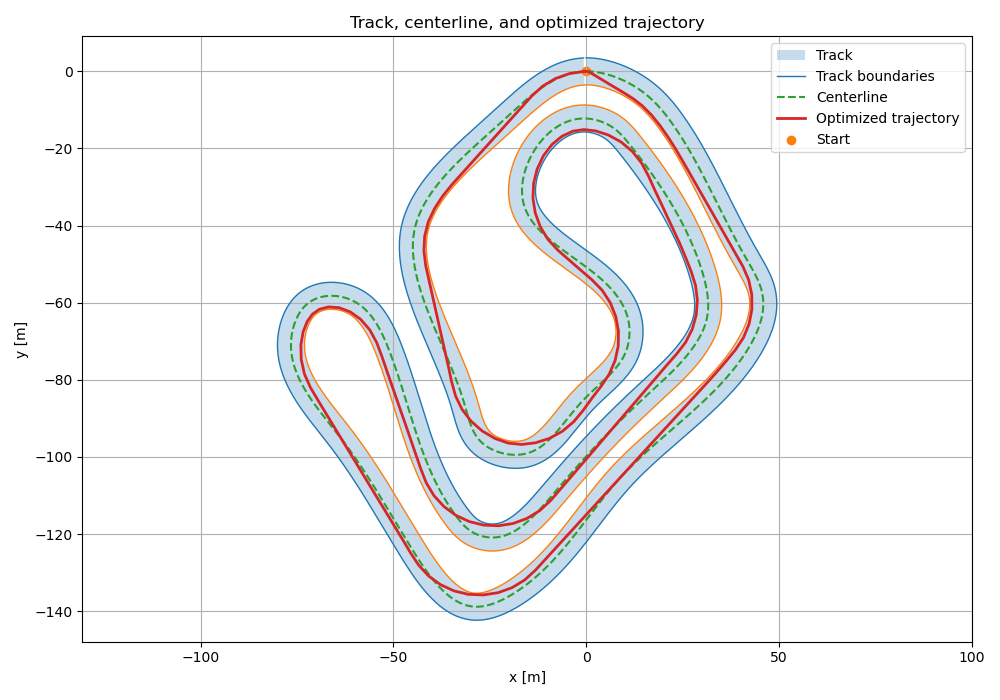
\includegraphics[width=0.70\linewidth]{images/track_optimzed_traj.png}
    \caption{Reconstructed track geometry, centerline and optimized trajectory.}
    \label{fig:trajectory}
\end{figure}

The corresponding lateral displacement is shown in Figure~\ref{fig:lateral}. The optimizer makes use of almost the entire admissible width, reaching the limits of \(\pm2.87~\mathrm{m}\) in several corners. This behaviour is consistent with an optimal racing line, where the vehicle moves towards the outside before entering a corner and approaches the inside near the apex.

\begin{figure}[htbp]
    \centering
    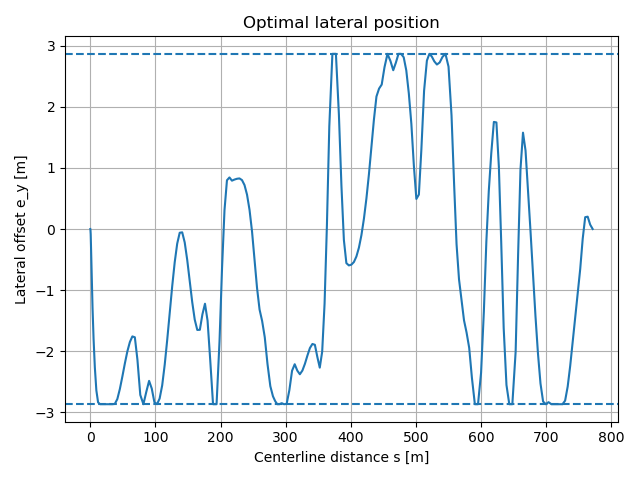
\includegraphics[width=0.70\linewidth]{images/opt_lat_pos.png}
    \caption{Optimized lateral displacement with admissible track limits.}
    \label{fig:lateral}
\end{figure}

The optimal velocity profile is presented in Figure~\ref{fig:velocity}. The kart rapidly accelerates to the maximum allowed speed of \(12.5~\mathrm{m/s}\) and remains close to this value over most of the circuit. Speed reductions only occur in the sections with the highest curvature, where the lateral-acceleration constraint becomes active.

\begin{figure}[htbp]
    \centering
    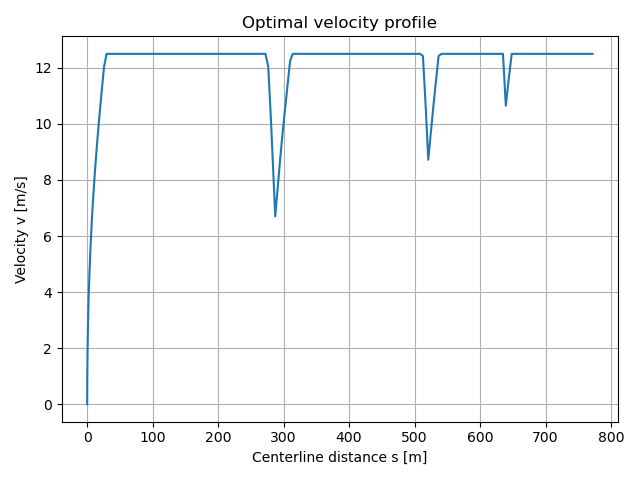
\includegraphics[width=0.70\linewidth]{images/vel_profile.png}
    \caption{Optimal velocity profile along the track centerline.}
    \label{fig:velocity}
\end{figure}

The longitudinal acceleration varies between \(-6.0\) and \(3.0~\mathrm{m/s^2}\), while the lateral acceleration reaches the imposed limits of \(\pm8.0~\mathrm{m/s^2}\). This indicates that both the longitudinal and lateral capabilities of the vehicle are fully exploited during the lap. The steering angle remains within the prescribed bounds, ranging from \(-0.600\) to \(0.126~\mathrm{rad}\).

Finally, the minimum value of the Frenet-coordinate denominator is

\[
\min(1-\kappa e_y)=0.6827,
\]

which remains well above zero throughout the optimization. Therefore, the computed trajectory stays within the valid region of the Frenet-coordinate formulation.